\DiaryEntry{NTP / Clock Sync}{2020-10-23}{General}

\subsection{Introduction}

The "NTP homepage" \href{https://www.eecis.udel.edu/~mills/ntp.html}{here} has some good slides. Basically, NTP is used to align / synchronize clocks of computers in a network with round-trip delay. There are several operation modes such client-server (where the client wants to synchronize its clock to the server's) and peer-to-peer where several servers synchronize their clocks. We concentrate on the simple client-server model.

NTP exchanges UDP packets which have the following form (taken from \href{https://www.eecis.udel.edu/~mills/database/brief/arch/arch.pdf}{here}).

\begin{figure}[H]
    \centering
    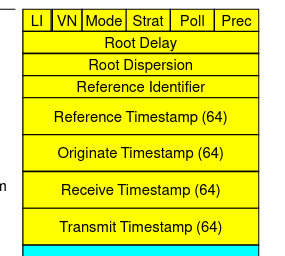
\includegraphics[scale=0.75]{images/ntp_1.png}
\end{figure}

Most important are the four timestamps: reference timestamp, originate timestamp, receive timestamps, and transmit timestamp. Two timestamps are filled out by the client (when the NTP packet is sent and received); the other two fields are filled out by the server (when the NTP is received and sent back). Using these four timestamps, the client can adjust its clock as described in the following.

\subsection{Principle of Operation}

We have two computers A and B, each having their own clock. The clocks have the same period (that's one assumption) but are shifted by some time offset $\theta$. The computers are connected via a network (IP) introducing some delay when the computer exchange NTP packets.

Ad time offset: Assume the operators at the two computers observe the same event (e.g. flash of lightning). When they look at their computer's clock, the difference of the clocks is $\theta$.

\paragraph{Definition Round-trip Delay.} Assume computer A sends a packet to computer B at time $t_0$; i.e. compter A's clock shows $t_0$ at time of sending. The packet is received when computer B's clock shows time $t_1$. Now the server processes the packet and sends it back at computer B's time $t_2$ and it is received at computer A's time $t_3$. The time the packet spent on the network is defined as round-trip delay $\delta$ and given by

\bee
\delta = t_3 - t_0 - (t_2 - t_1)
\eee

Note that it does not matter that computer A's clock has an offset to computer B's clock; we are only interested in time differences, therefore the time offset $\theta$ is not relevant here.

\paragraph{Time Shift.} Now let's concentrate on what happens when computer A sends the packet: It is sent at computer A's time $t_0$, then it spends $\delta/2$ time on the network (assuming the network delay is the same in both directions, namely $\delta/2$); at time of reception computer B's time shows $t_1$ which is shifted by $\theta$ from computer A's time. We therefore have

\be\label{eq:ntp_1}
t_1 = t_0 + \delta/2 + \theta
\ee

The same happens in the other direction; at time $t_2$ computer B sends the packet, it spends $\delta/2$ on the network and is received at computer B's time $t_3$. We therefore have

\bee
t_3 = t_2 + \delta/2 - \theta
\eee

Note that in this case the time offset works in the "other direction"; i.e. $\theta$ is subtracted to get from computer B's time to computer A's time. We can rewrite and obtain

\be\label{eq:ntp_2}
t_2 = t_3 - \delta/2 + \theta
\ee

Adding the last equation to \eqref{eq:ntp_1} yields

\bee
t_1 + t_2 = t_0 + \theta + t_3 + \theta
\eee

Luckily the network delay has cancelled and we obtain for the time offset

\bee
\theta = \frac{(t_1 - t_0) + (t_2 - t_3)}{2}
\eee


\subsection{Extensions, Further Thoughts}

What happens when the round-trip delay is different in each direction? Then we have two unequal delays $\delta \neq \delta_2$ summing up as $\delta_1 + \delta_2 = \delta$. However, adding \eqref{eq:ntp_1} and \eqref{eq:ntp_2} does not cancel the delays. \todo{Are there other operation modes wich help in this case?}

We have assumed that the clocks have the same period and have only a time shift. What happens if the clock period is different? As a first consequence the time shift becomes time dependent; i.e. we have $\theta = \theta(t)$ and the magic in above equations does not work either. Not sure, however, whether this is relevant as the times $t_0 \cdots t_3$ are typcially small (less than a second) and the clock period difference is much higher (clocks maybe differ in a couple of seconds per day) - this should not matter.


%%% Local Variables:
%%% mode: latex
%%% TeX-master: "journal"
%%% End:
